\documentclass{standalone}
\usepackage{tikz}
\usetikzlibrary{patterns, positioning}
\usepackage[sfdefault]{ClearSans} %% option 'sfdefault' activates Clear Sans as the default text font
\usepackage[T1]{fontenc}

\begin{document}
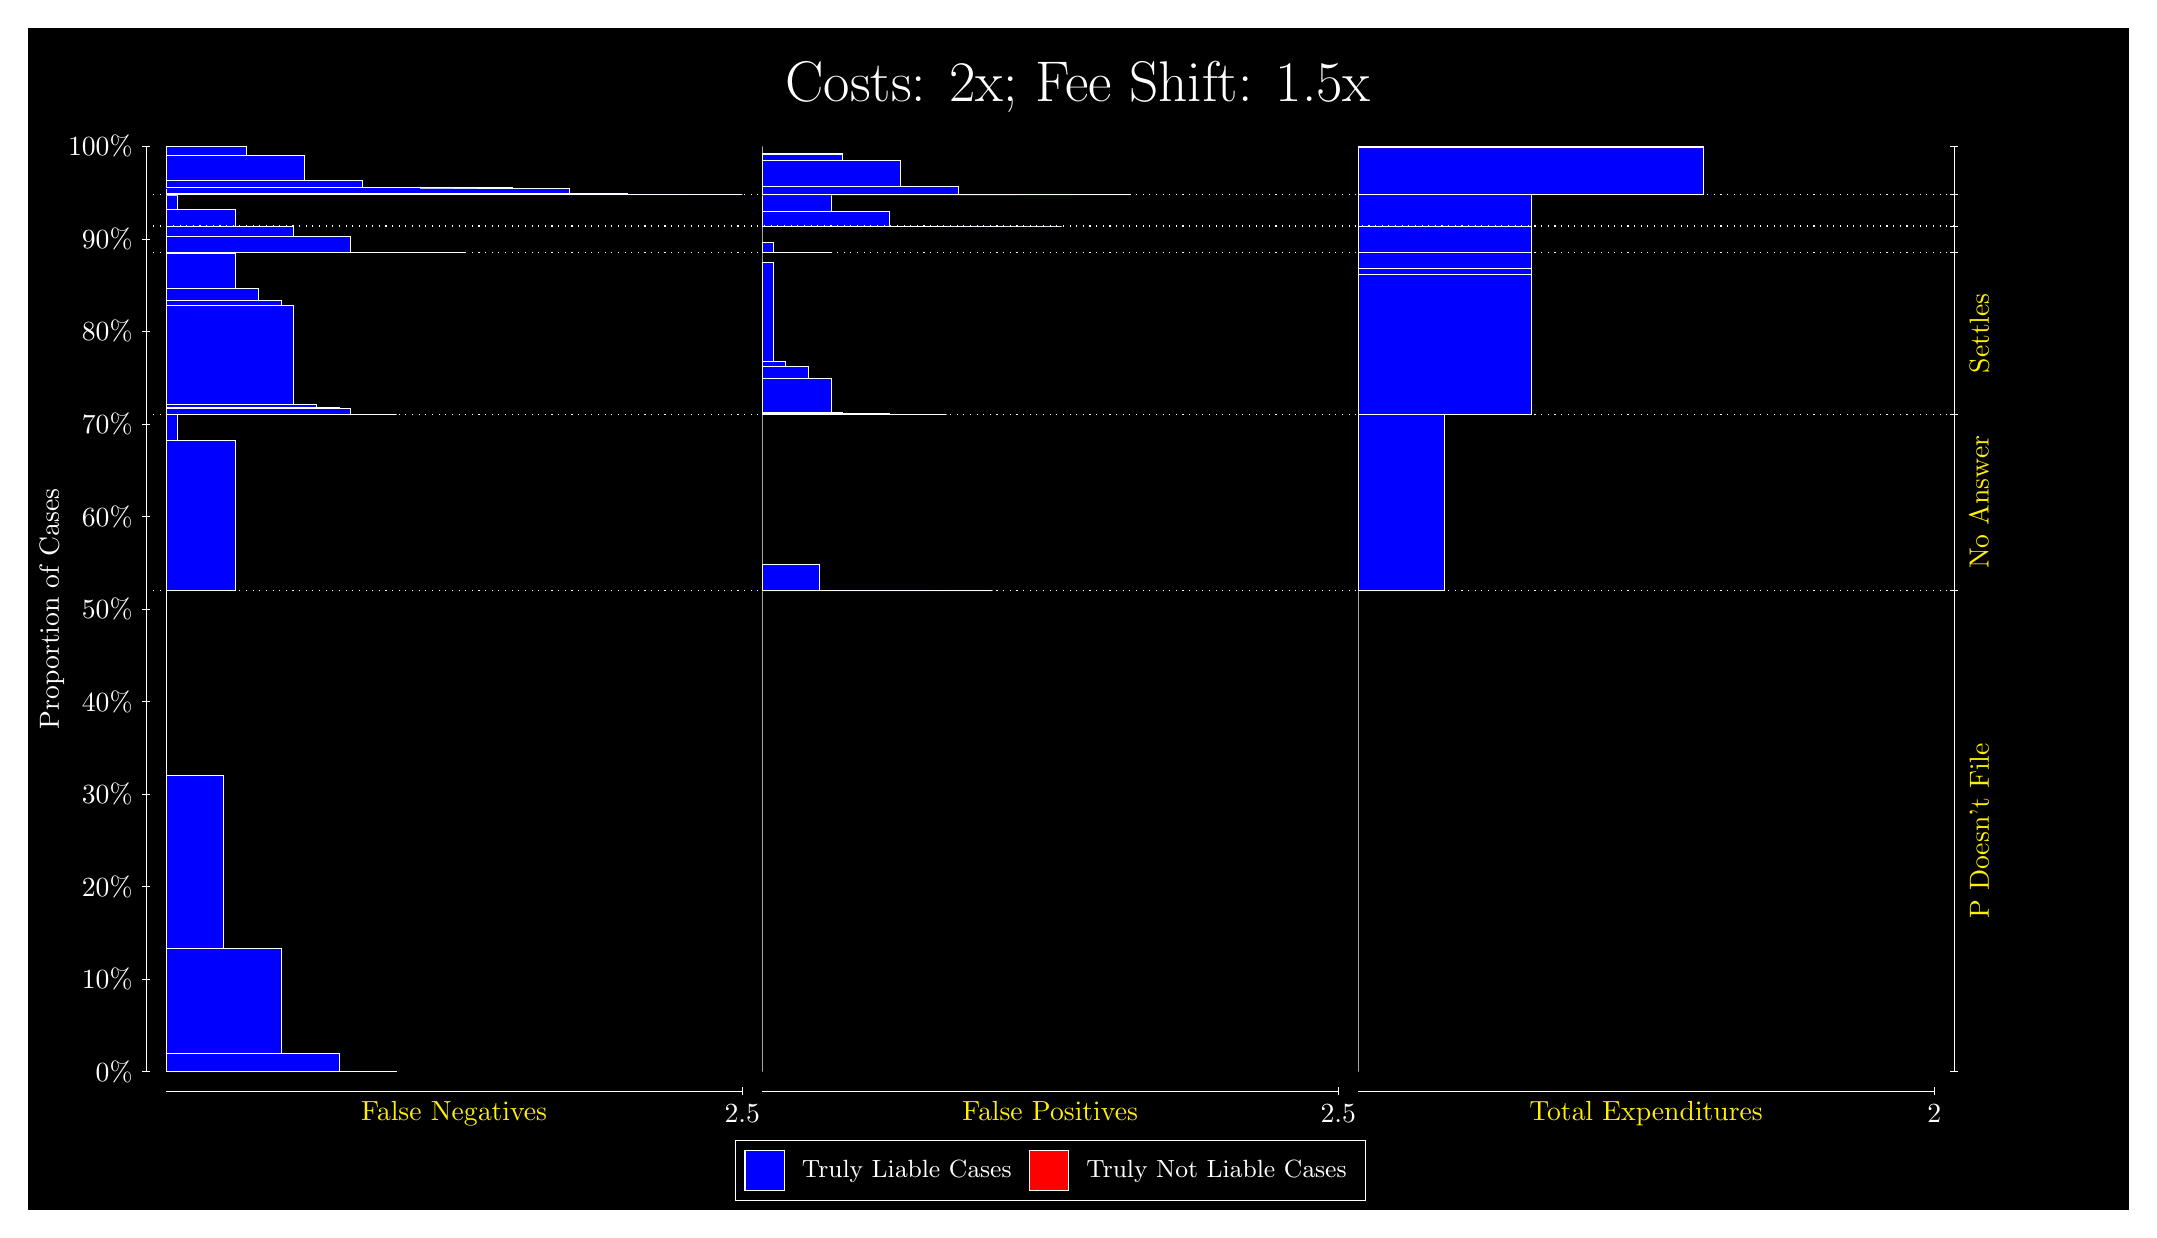
\begin{tikzpicture}
\draw[fill=black] (0,0) rectangle (26.667,15);
\draw[text=white] (0,13.5) rectangle (26.667,15) node[midway] {\huge Costs: 2x; Fee Shift: 1.5x};
\draw[white, very thin] (1.5,1.75) -- (1.5,13.5);
\node[rotate=90, text=white, anchor=center] at (0.3, 7.625) {Proportion of Cases};
\draw[white, very thin] (1.45,1.75) -- (1.55,1.75);
\node[text=white, anchor=east] at (1.45, 1.75) {0\%};
\draw[white, very thin] (1.45,2.925) -- (1.55,2.925);
\node[text=white, anchor=east] at (1.45, 2.925) {10\%};
\draw[white, very thin] (1.45,4.1) -- (1.55,4.1);
\node[text=white, anchor=east] at (1.45, 4.1) {20\%};
\draw[white, very thin] (1.45,5.275) -- (1.55,5.275);
\node[text=white, anchor=east] at (1.45, 5.275) {30\%};
\draw[white, very thin] (1.45,6.45) -- (1.55,6.45);
\node[text=white, anchor=east] at (1.45, 6.45) {40\%};
\draw[white, very thin] (1.45,7.625) -- (1.55,7.625);
\node[text=white, anchor=east] at (1.45, 7.625) {50\%};
\draw[white, very thin] (1.45,8.8) -- (1.55,8.8);
\node[text=white, anchor=east] at (1.45, 8.8) {60\%};
\draw[white, very thin] (1.45,9.975) -- (1.55,9.975);
\node[text=white, anchor=east] at (1.45, 9.975) {70\%};
\draw[white, very thin] (1.45,11.15) -- (1.55,11.15);
\node[text=white, anchor=east] at (1.45, 11.15) {80\%};
\draw[white, very thin] (1.45,12.325) -- (1.55,12.325);
\node[text=white, anchor=east] at (1.45, 12.325) {90\%};
\draw[white, very thin] (1.45,13.5) -- (1.55,13.5);
\node[text=white, anchor=east] at (1.45, 13.5) {100\%};

\draw[white, very thin] (24.457,1.75) -- (24.457,13.5);
\draw[white, very thin] (24.407,1.75) -- (24.507,1.75);
\node[anchor=west] at (24.407, 1.75) {};
\draw[white, very thin] (24.407,7.8581) -- (24.507,7.8581);
\node[anchor=west] at (24.407, 7.8581) {};
\draw[white, very thin] (24.407,10.099) -- (24.507,10.099);
\node[anchor=west] at (24.407, 10.099) {};
\draw[white, very thin] (24.407,12.155) -- (24.507,12.155);
\node[anchor=west] at (24.407, 12.155) {};
\draw[white, very thin] (24.407,12.488) -- (24.507,12.488);
\node[anchor=west] at (24.407, 12.488) {};
\draw[white, very thin] (24.407,12.887) -- (24.507,12.887);
\node[anchor=west] at (24.407, 12.887) {};
\draw[white, very thin] (24.407,13.5) -- (24.507,13.5);
\node[anchor=west] at (24.407, 13.5) {};

\draw[white, very thin, fill=blue] (1.75,1.75) rectangle (4.6775,1.7523);
\draw[white, very thin, fill=blue] (1.75,1.7523) rectangle (3.9457,1.9772);
\draw[white, very thin, fill=blue] (1.75,1.9772) rectangle (3.2138,3.3111);
\draw[white, very thin, fill=blue] (1.75,3.3111) rectangle (2.4819,5.5096);
\draw[white, very thin, fill=red] (1.75,5.5096) rectangle (1.75,5.5096);
\draw[white, very thin, fill=blue] (1.75,5.5096) rectangle (1.75,7.8581);
\draw[white, very thin, fill=blue] (1.75,7.8581) rectangle (2.6283,9.763);
\draw[white, very thin, fill=blue] (1.75,9.763) rectangle (1.8964,10.098);
\draw[white, very thin, fill=red] (1.75,10.098) rectangle (1.75,10.098);
\draw[white, very thin, fill=blue] (1.75,10.098) rectangle (1.75,10.099);
\draw[white, very thin, fill=blue] (1.75,10.099) rectangle (4.6775,10.099);
\draw[white, very thin, fill=blue] (1.75,10.099) rectangle (4.3848,10.099);
\draw[white, very thin, fill=blue] (1.75,10.099) rectangle (4.092,10.177);
\draw[white, very thin, fill=blue] (1.75,10.177) rectangle (3.9457,10.181);
\draw[white, very thin, fill=blue] (1.75,10.181) rectangle (3.6529,10.228);
\draw[white, very thin, fill=blue] (1.75,10.228) rectangle (3.3602,11.483);
\draw[white, very thin, fill=blue] (1.75,11.483) rectangle (3.2138,11.546);
\draw[white, very thin, fill=blue] (1.75,11.546) rectangle (2.921,11.702);
\draw[white, very thin, fill=blue] (1.75,11.702) rectangle (2.6283,12.136);
\draw[white, very thin, fill=blue] (1.75,12.136) rectangle (2.4819,12.14);
\draw[white, very thin, fill=blue] (1.75,12.14) rectangle (2.1891,12.146);
\draw[white, very thin, fill=blue] (1.75,12.146) rectangle (1.8964,12.155);
\draw[white, very thin, fill=red] (1.75,12.155) rectangle (1.75,12.155);
\draw[white, very thin, fill=blue] (1.75,12.155) rectangle (1.75,12.155);
\draw[white, very thin, fill=blue] (1.75,12.155) rectangle (5.5558,12.155);
\draw[white, very thin, fill=blue] (1.75,12.155) rectangle (4.8239,12.16);
\draw[white, very thin, fill=blue] (1.75,12.16) rectangle (4.092,12.357);
\draw[white, very thin, fill=blue] (1.75,12.357) rectangle (3.3602,12.487);
\draw[white, very thin, fill=blue] (1.75,12.487) rectangle (2.6283,12.488);
\draw[white, very thin, fill=red] (1.75,12.488) rectangle (1.75,12.488);
\draw[white, very thin, fill=blue] (1.75,12.488) rectangle (2.6283,12.699);
\draw[white, very thin, fill=blue] (1.75,12.699) rectangle (1.8964,12.884);
\draw[white, very thin, fill=red] (1.75,12.884) rectangle (1.75,12.884);
\draw[white, very thin, fill=blue] (1.75,12.884) rectangle (1.75,12.887);
\draw[white, very thin, fill=blue] (1.75,12.887) rectangle (9.0689,12.887);
\draw[white, very thin, fill=blue] (1.75,12.887) rectangle (8.337,12.887);
\draw[white, very thin, fill=blue] (1.75,12.887) rectangle (7.6051,12.902);
\draw[white, very thin, fill=blue] (1.75,12.902) rectangle (6.8732,12.968);
\draw[white, very thin, fill=blue] (1.75,12.968) rectangle (6.1413,12.974);
\draw[white, very thin, fill=blue] (1.75,12.974) rectangle (5.7022,12.974);
\draw[white, very thin, fill=blue] (1.75,12.974) rectangle (5.4094,12.974);
\draw[white, very thin, fill=blue] (1.75,12.974) rectangle (4.9703,12.975);
\draw[white, very thin, fill=blue] (1.75,12.975) rectangle (4.6775,12.975);
\draw[white, very thin, fill=blue] (1.75,12.975) rectangle (4.2384,13.063);
\draw[white, very thin, fill=blue] (1.75,13.063) rectangle (3.5065,13.389);
\draw[white, very thin, fill=blue] (1.75,13.389) rectangle (2.7746,13.496);
\draw[white, very thin, fill=blue] (1.75,13.496) rectangle (2.0428,13.5);
\draw[white, very thin, fill=red] (1.75,13.5) rectangle (1.75,13.5);
\draw[white, very thin, fill=blue] (1.75,13.5) rectangle (1.75,13.5);
\draw[white, very thin, fill=red] (9.3189,1.75) rectangle (9.3189,1.75);
\draw[white, very thin, fill=blue] (9.3189,1.75) rectangle (9.3189,7.8581);
\draw[white, very thin, fill=red] (9.3189,7.8581) rectangle (12.246,7.8581);
\draw[white, very thin, fill=blue] (9.3189,7.8581) rectangle (12.246,7.8581);
\draw[white, very thin, fill=blue] (9.3189,7.8581) rectangle (11.515,7.8581);
\draw[white, very thin, fill=blue] (9.3189,7.8581) rectangle (10.783,7.8594);
\draw[white, very thin, fill=blue] (9.3189,7.8594) rectangle (10.051,8.1942);
\draw[white, very thin, fill=blue] (9.3189,8.1942) rectangle (9.3189,10.099);
\draw[white, very thin, fill=red] (9.3189,10.099) rectangle (11.661,10.099);
\draw[white, very thin, fill=blue] (9.3189,10.099) rectangle (11.661,10.099);
\draw[white, very thin, fill=red] (9.3189,10.099) rectangle (11.368,10.099);
\draw[white, very thin, fill=blue] (9.3189,10.099) rectangle (11.368,10.099);
\draw[white, very thin, fill=red] (9.3189,10.099) rectangle (11.075,10.099);
\draw[white, very thin, fill=blue] (9.3189,10.099) rectangle (11.075,10.099);
\draw[white, very thin, fill=blue] (9.3189,10.099) rectangle (10.929,10.108);
\draw[white, very thin, fill=blue] (9.3189,10.108) rectangle (10.636,10.115);
\draw[white, very thin, fill=blue] (9.3189,10.115) rectangle (10.344,10.118);
\draw[white, very thin, fill=blue] (9.3189,10.118) rectangle (10.197,10.552);
\draw[white, very thin, fill=blue] (9.3189,10.552) rectangle (9.9044,10.708);
\draw[white, very thin, fill=blue] (9.3189,10.708) rectangle (9.6116,10.771);
\draw[white, very thin, fill=blue] (9.3189,10.771) rectangle (9.4652,12.026);
\draw[white, very thin, fill=blue] (9.3189,12.026) rectangle (9.3189,12.155);
\draw[white, very thin, fill=red] (9.3189,12.155) rectangle (10.197,12.155);
\draw[white, very thin, fill=blue] (9.3189,12.155) rectangle (10.197,12.157);
\draw[white, very thin, fill=blue] (9.3189,12.157) rectangle (9.4652,12.287);
\draw[white, very thin, fill=blue] (9.3189,12.287) rectangle (9.3189,12.488);
\draw[white, very thin, fill=red] (9.3189,12.488) rectangle (13.125,12.488);
\draw[white, very thin, fill=blue] (9.3189,12.488) rectangle (13.125,12.488);
\draw[white, very thin, fill=blue] (9.3189,12.488) rectangle (12.393,12.488);
\draw[white, very thin, fill=blue] (9.3189,12.488) rectangle (11.661,12.49);
\draw[white, very thin, fill=blue] (9.3189,12.49) rectangle (10.929,12.676);
\draw[white, very thin, fill=blue] (9.3189,12.676) rectangle (10.197,12.887);
\draw[white, very thin, fill=red] (9.3189,12.887) rectangle (14.003,12.887);
\draw[white, very thin, fill=blue] (9.3189,12.887) rectangle (14.003,12.887);
\draw[white, very thin, fill=red] (9.3189,12.887) rectangle (13.271,12.887);
\draw[white, very thin, fill=blue] (9.3189,12.887) rectangle (13.271,12.887);
\draw[white, very thin, fill=red] (9.3189,12.887) rectangle (12.539,12.887);
\draw[white, very thin, fill=blue] (9.3189,12.887) rectangle (12.539,12.89);
\draw[white, very thin, fill=blue] (9.3189,12.89) rectangle (11.807,12.997);
\draw[white, very thin, fill=red] (9.3189,12.997) rectangle (11.807,12.997);
\draw[white, very thin, fill=blue] (9.3189,12.997) rectangle (11.807,12.997);
\draw[white, very thin, fill=blue] (9.3189,12.997) rectangle (11.075,13.323);
\draw[white, very thin, fill=blue] (9.3189,13.323) rectangle (11.075,13.324);
\draw[white, very thin, fill=blue] (9.3189,13.324) rectangle (10.344,13.398);
\draw[white, very thin, fill=blue] (9.3189,13.398) rectangle (10.344,13.412);
\draw[white, very thin, fill=red] (9.3189,13.412) rectangle (9.9044,13.412);
\draw[white, very thin, fill=blue] (9.3189,13.412) rectangle (9.9044,13.412);
\draw[white, very thin, fill=blue] (9.3189,13.412) rectangle (9.6116,13.412);
\draw[white, very thin, fill=blue] (9.3189,13.412) rectangle (9.6116,13.412);
\draw[white, very thin, fill=red] (9.3189,13.412) rectangle (9.3189,13.412);
\draw[white, very thin, fill=blue] (9.3189,13.412) rectangle (9.3189,13.5);
\draw[white, very thin, fill=red] (16.888,1.75) rectangle (16.888,1.75);
\draw[white, very thin, fill=blue] (16.888,1.75) rectangle (16.888,7.8581);
\draw[white, very thin, fill=red] (16.888,7.8581) rectangle (17.986,7.8581);
\draw[white, very thin, fill=blue] (16.888,7.8581) rectangle (17.986,10.099);
\draw[white, very thin, fill=red] (16.888,10.099) rectangle (19.083,10.099);
\draw[white, very thin, fill=blue] (16.888,10.099) rectangle (19.083,11.876);
\draw[white, very thin, fill=red] (16.888,11.876) rectangle (19.083,11.876);
\draw[white, very thin, fill=blue] (16.888,11.876) rectangle (19.083,11.946);
\draw[white, very thin, fill=red] (16.888,11.946) rectangle (19.083,11.946);
\draw[white, very thin, fill=blue] (16.888,11.946) rectangle (19.083,12.155);
\draw[white, very thin, fill=red] (16.888,12.155) rectangle (19.083,12.155);
\draw[white, very thin, fill=blue] (16.888,12.155) rectangle (19.083,12.488);
\draw[white, very thin, fill=red] (16.888,12.488) rectangle (19.083,12.488);
\draw[white, very thin, fill=blue] (16.888,12.488) rectangle (19.083,12.887);
\draw[white, very thin, fill=red] (16.888,12.887) rectangle (21.279,12.887);
\draw[white, very thin, fill=blue] (16.888,12.887) rectangle (21.279,13.485);
\draw[white, very thin, fill=red] (16.888,13.485) rectangle (21.279,13.485);
\draw[white, very thin, fill=blue] (16.888,13.485) rectangle (21.279,13.5);
\draw[white, dotted] (1.5,7.8581) -- (24.457,7.8581);
\draw[white, dotted] (1.5,10.099) -- (24.457,10.099);
\draw[white, dotted] (1.5,12.155) -- (24.457,12.155);
\draw[white, dotted] (1.5,12.488) -- (24.457,12.488);
\draw[white, dotted] (1.5,12.887) -- (24.457,12.887);
\draw[white, very thin] (1.75,1.5) -- (9.0689,1.5);
\node[text=yellow, anchor=north] at (5.4094, 1.5) {False Negatives};
\draw[white, very thin] (9.0689,1.45) -- (9.0689,1.55);
\node[text=white, anchor=north] at (9.0689, 1.45) {2.5};

\draw[white, very thin] (9.3189,1.5) -- (16.638,1.5);
\node[text=yellow, anchor=north] at (12.978, 1.5) {False Positives};
\draw[white, very thin] (16.638,1.45) -- (16.638,1.55);
\node[text=white, anchor=north] at (16.638, 1.45) {2.5};

\draw[white, very thin] (16.888,1.5) -- (24.207,1.5);
\node[text=yellow, anchor=north] at (20.547, 1.5) {Total Expenditures};
\draw[white, very thin] (24.207,1.45) -- (24.207,1.55);
\node[text=white, anchor=north] at (24.207, 1.45) {2};

\node[text=yellow, centered, rotate=90] at (24.777, 4.804) {P Doesn't File};
\node[text=yellow, centered, rotate=90] at (24.777, 8.9786) {No Answer};
\node[text=yellow, centered, rotate=90] at (24.777, 11.127) {Settles};




\draw (12.978300999999998,1.5) node[draw=none] (baseCoordinate) {};
\begin{scope}[align=center]
        \matrix[scale=0.5, draw=white, below=0.5cm of baseCoordinate, nodes={draw}, column sep=0.1cm]{
            \node[rectangle, draw, minimum width=0.5cm, minimum height=0.5cm, fill=blue] {}; &
            \node[draw=none, font=\small, text=white] (B) {Truly Liable Cases}; &
            \node[rectangle, draw, minimum width=0.5cm, minimum height=0.5cm, fill=red] {}; &
            \node[draw=none, font=\small, text=white] (B) {Truly Not Liable Cases}; \\
            };
\end{scope}

\end{tikzpicture}
\end{document}